\chapter{The LHC and CMS Machine} % (fold)
\label{cha:the_lhc_and_cms_machine}

In this chapter, the working and the design parameters of \acrfull{lhc} and its one of main purpose detector, Compact Muon Solenoid (CMS), is briefly described.


%%%%%%%%%%%%%%%%%%%%%%%%%%%%%%%%%%%%%%%%%%%%%%%%%%%%%%%%%%%%%%%%%%
\section{The Large Hadron Collider} % (fold)
\label{sec:the_large_hadron_collider}

The famous quote ``history repeats itself" applies well to the \acrfull{hep} experiments. The starting point of experimental particle physics is the Rutherford $\alpha$-particle scattering, and even now we are doing the same thing just the method changed from ``natural accelerator" to the ``man-made" accelerator that can accelerate particles with the velocity close to the speed of light. The design and working of accelerator changed a lot over a period of time in going from MeV to GeV and in the TeV range. Now, these machines are not only used in \acrshort{hep} experiments, but extends its arena to treat human beings like cancer therapy, radioisotope production, 3-D x-ray\todo[fancyline]{Add citations to the applications}, also to the industry for uses like material processing, sterilization, security scan, water treatment, and many more. 

The \acrshort{lhc} is  a hadron collider which can accelerate the two proton beams in opposite direction with maximum of 14 TeV energy in a 26.6 km long tunnel which is about 100 m underground. The \acrshort{lhc} is the latest and most-powerful accelerator everbuilt. It is a proton-proton collider built to improve our understanding of fundamental physics. It started on 21$^{st}$ October 2008. It is built in the same tunnel where there was Large Electron Positron (LEP) collider, that collides electrons and positrons. LEP collaboration decided to switch to hadron collider because of following advantages:
\begin{itemize}
    \item Hadron collider can reach a higher Center Of Mass (COM) energy, because of much lower synchrotron radiation \footnote{The radiation emitted by charged particle during acceleration in a circular path is known as synchrotron radiation. As the particlee will loose energy with this so we must provide the additional energy to keep the beam at constant energy.} emitted by hadrons as compared to electrons. Synchrotron radiation loss is directory proportional to $(Energy/mass)^4$. \todo[fancyline]{Add exact number for electrons and protons synchrotron loss.}
    \item As hadrons are composite particles so it allows us to scan over wide range of energy.
\end{itemize}


For any particle accelerator there are mainly three components so for the LHC. They are:
\begin{itemize}
  \item Beam pipes
  \item Accelerating structure
  \item Magnet system
\end{itemize}

%%%%%%%%%%%%%%%%%%%%%%%%%%%%%%%%%%%%%%%%%%%%%%%%%%%%%%%%%%%%%%%%%%
%%%%%%%%%%%%%%%%%%%%%%%%%%%%%%%%%%%%%%%%%%%%%%%%%%%%%%%%%%%%%%%%%%
\subsection{Beam Pipes} % (fold)
\label{sub:beam_pipes}

At LHC there are two beam pipes each with diameter $\approx$6.3 cm in which proton beam travels in opposite direction. We should keep the beam pipes with ultra-high vacuum\footnote{At LHC there are three different vacuum systems used. First one is used for beam pipe another is used for insulating the cryogenically cooled magnets and third one is used for insulating the helium distribution. In the later two it it just acts as a thermal insulator as the cryogenic parts are kept at 1.9 K ($\ang{-271.3}C$)} to minimize the number of collision with the gas molecules which result in beam instability and loss of beam particles. At LHC the beam pipes are kept at $1.013 \times 10^{-13}$ bar pressure.
% subsection beam_pipes (end)

%%%%%%%%%%%%%%%%%%%%%%%%%%%%%%%%%%%%%%%%%%%%%%%%%%%%%%%%%%%%%%%%%%
%%%%%%%%%%%%%%%%%%%%%%%%%%%%%%%%%%%%%%%%%%%%%%%%%%%%%%%%%%%%%%%%%%
\subsection{Accelerating Structure} % (fold)
\label{sub:accelerating_structure}

Another main part of any particle accelerator is its accelerating structure. A accelerator in TeV range can not start from rest and go to the TeV range in one go it should go into several stages depending on the energy. At LHC the journey of proton starts from grabbing the proton from Hydrogen gas and subsequently go into 5 different stages. The stages can be decreased but could not be just one stage. Here, at LHC there are five different stages before reaching to LHC as in between it serves several other experiments at each stage, which are shown pictorially in Figure~\ref{fig:OtherExpAtAccStructure}. The stages for proton acceleration are:
\begin{itemize}
    \item Grab proton source: The source of proton is Duoplasmatron\footnote{It strips electron from hydrogen gas and creates a plasma of protons, electrons and molecular ions. This plasma expands towards the extraction electrodes and a proton beam is formed}\cite{LHC-tdr-vol3}. This feed protons to LINAC2.
    \item LINAC2 (Linear accelerator-2): It is the starting point of proton's journey in the LHC accelerator complex. Here, protons reaches to an energy of 50 $MeV$ using the radio-frequency (RF) cavities\footnote{A RF cavity is an metallic cavity that accelerates the charged particles using the electromagnetic field.} where it also gains 5\% in mass. It feeds to the Proton Synchrotron Booster (PSB).
    \item PSB: It takes 50 $MeV$ protons beams from LINAC2 and accelerates it to 1.4 $GeV$ for the injection into Proton Synchrotron (PS).
    \item PS: It is one of key component in the LHC accelerator complex. It increases the energy of protons up-to 25 $GeV$ and feeds to super proton synchrotron.
    \item Super Proton Synchrotron (SPS): It has a circumference of 7 $km$ where protons are accelerated to an energy of 450 $GeV$. Then via two transmission line protons are then injected into LHC ring.
    \item LHC: It grabs two proton beams from SPS which is injected into opposite direction in parallel pipes. In LHC proton beams can be accelerated up-to 7 $TeV$.
\end{itemize}
The CERN accelerator complex is shown in Figure~\ref{fig:CERN-accelerator-complex}.  

% subsection accelerating_structure (end)
\begin{figure}[!htbp]
	\centering
	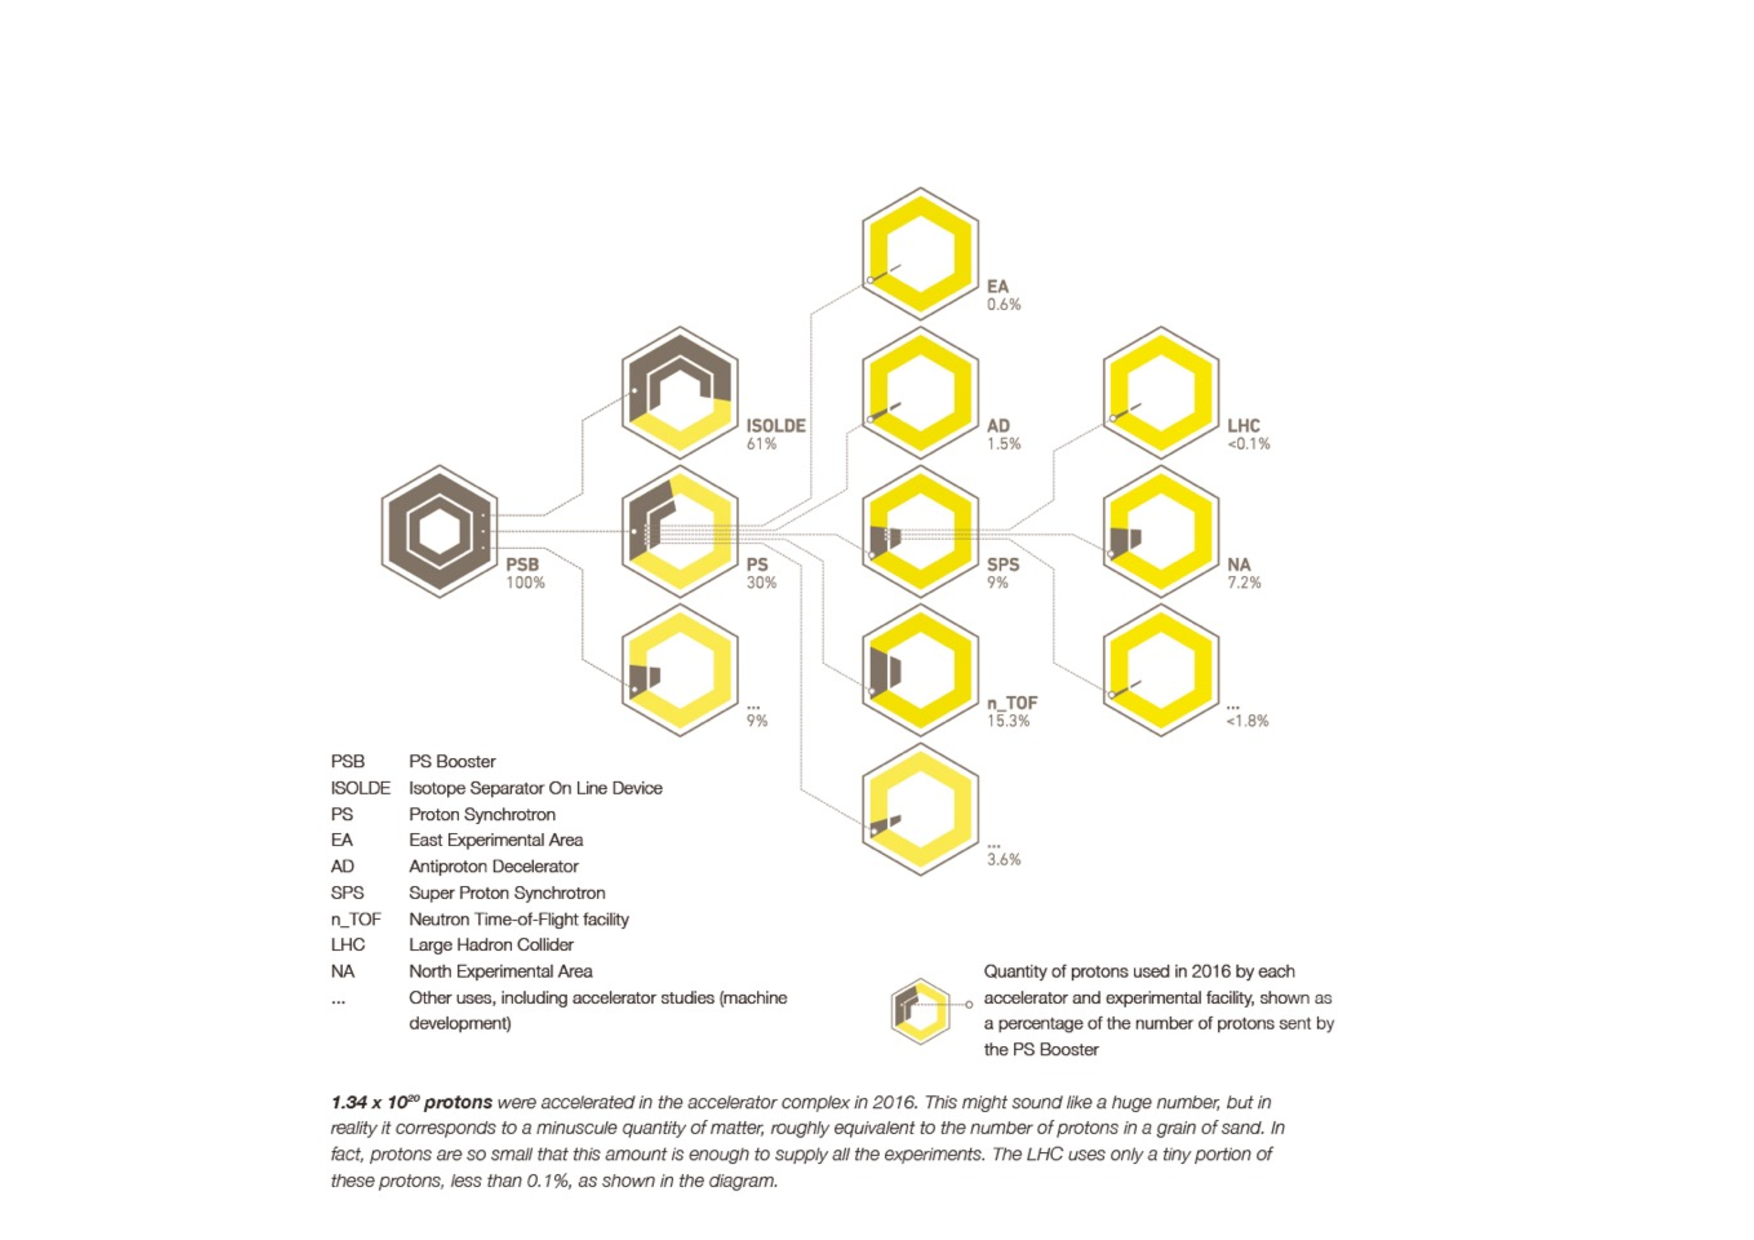
\includegraphics[width=1.0\textwidth]{figures/LHC/distribution_of_protons_en.pdf}
	\caption{Other experiments at the LHC accelerating chain \cite{OtherExpAtLHCAcceleratingChain}}
	\label{fig:OtherExpAtAccStructure}
\end{figure}
\begin{figure}[!htbp]
	\centering
	\includegraphics[width=1.35\textwidth]{figures/CERN_Accelerator_Complex-v2016.pdf}
	\caption{LHC accelerator chain along with all its other experiments which uses proton beam from other part of accelerator either from PSB, PS or SPS\cite{Fig-CERN-accelerator-complex}}
	\label{fig:CERN-accelerator-complex}
\end{figure}
%%%%%%%%%%%%%%%%%%%%%%%%%%%%%%%%%%%%%%%%%%%%%%%%%%%%%%%%%%%%%%%%%%
%%%%%%%%%%%%%%%%%%%%%%%%%%%%%%%%%%%%%%%%%%%%%%%%%%%%%%%%%%%%%%%%%%
\subsection{Magnet System}
As the LHC is a circular collider so magnet system is its one of core part which give them a circular trajectory in the LHC beam pipes. %Apart from bending the beams magnet systems are also used to focus the beam and for making various corrections to the beam. 

To be economical LHC is made in eight arcs and eight straight sections instead of a perfect circle. Along with the bending of beam it is also necessary to focus the beam as the same charge protons try to diverge. To focus the beam a pair of quadrapole magnets are used one focuses the beam width while other focus the beam height. Quadrapole magnet geometry is shown in Figure~\ref{fig:QuadrupoleMagnet}. There are total of 858 quadrupole magnets are installed in LHC to keep the beam focused. Along with this every protons in the beam are not exactly with the same energy and in same path. To correct this focusing with change in energy there are sextupoles magnets are used. There are several other magnetic multi-poles are used that help us to keep beam focused if the beam suffers from gravitational interactions over protons, electromagnetic interactions among bunches, electron clouds from pipe wall, and so on. Different types of magnets used in LHC are listed here \cite{WebLink:LHC_magnets}. Along with this there are eight sets of ``inner triplets" are used. These are used at the four interaction points to focus the beam while collide to increase the luminosity. Here the size of bunch goes from 0.2 mm to 17 $\mu m$ at the interaction point of ATLAS or CMS. At the interaction point of ALICE or LHCb it is 71 $\mu m$. Summary of important parameters of LHC is given in Table~\ref{table:LHC-parameters}.
\begin{figure}[!htbp]
	\centering
	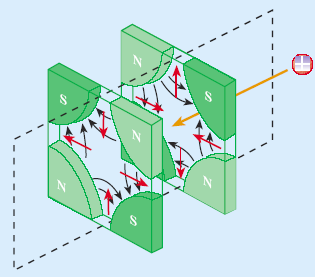
\includegraphics[width=0.65\textwidth]{figures/LHC/quadrupole_magnet_pair.png}
	\caption{Pair of quadrupole magnets.}
	\label{fig:QuadrupoleMagnet}
\end{figure}
% \begin{figure}[!htbp]
% 	\centering
% 	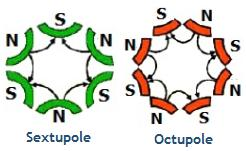
\includegraphics[width=0.95\textwidth]{figures/LHC/sextupole-octupole.jpg}
% 	\caption{Sextupole and octupole}
% 	\label{fig:sextupole-octupole}
% \end{figure}



\begin{table}
\centering
\begin{tabular}[!htbp]{l c}
\hline
{\bf Parameters} & {\bf Value} \\
\hline
Circumference of LHC ring   &   26658.883 m \\
\hline
Maximum dipole magnetic field   & 8.33 T \\
Dipole operating temperature    & 1.9 K \\
\hline
Maximum stored energy per beam (nominal) &   362 MJ \\
Maximum stored energy per beam  (2012) &   143 MJ \\
Maximum stored energy per beam  (2016) &   266 MJ \\
\hline
Beam energy at Injection    & 450 GeV \\
Beam energy at collision (nominal) &    7 TeV \\
Beam energy at collision (2012)     &   4 TeV \\
Beam energy at collision (2016)     &   6.5 TeV \\
\hline
Maximum instantaneous luminosity (nominal)  &   $10^{34}$ cm$^-2$ s$^{-1}$ \\
Maximum instantaneous luminosity (2012)     &   $7.7 \times 10^{33}$ cm$^-2$ s$^{-1}$ \\
Maximum instantaneous luminosity (2016)     &   $1.4 \times 10^{34}$ cm$^-2$ s$^{-1}$ \\
\hline
Number of bunches per proton beam (nominal) &   2808 \\
Number of bunches per proton beam (2012)    &   1380 \\
Number of bunches per proton beam (2016)    &   2076 \\
Maximum number of protons per bunch         &   $1.6 \times 10^{11}$ \\
\hline
Protons/bunch (average at start of collision) (nominal)   &   $1.15 \times 10^{11}$ \\
Protons/bunch (average at start of collision) (2012)  &   $1.5 \times 10^{11}$ \\
Protons/bunch (average at start of collision) (2016)  &   $1.1 \times 10^{11}$ \\
\hline
Bunch collision frequency (nominal)         &   40 MHz  \\
Bunch collision frequency (2012)            &   20 MHz  \\
Bunch collision frequency (2016)            &   40 MHz  \\
\hline
Bunch length (at injection)   &   1.7 ns \\
Bunch length (at collision)   &   1.05 ns \\
Energy spread (at injection)   &   1.9$\times 10^{-3}$ \\
Energy spread (at collision)   &   0.45$\times 10^{-3}$  \\
\hline
Half crossing angle  (nominal)   & 143 $\mu rad$ \\
Half crossing angle  (2012)   & 146 $\mu rad$ \\
Half crossing angle  (2016)   & 185 $\mu rad$ \\
\hline
$\beta *$  (nominal) &   0.55 m\\
$\beta *$   (2012)&   0.6 m\\
$\beta *$   (2016)&   0.4 m\\
\hline
RMS beam size at IP1 \& IP5 &   17 $\mu m$ \\
RMS beam size at IP2 \& IP8 &   71 $\mu m$ \\
\hline
$\epsilon_n$(transverse emittance, rms, normalized) (at injection) &   3.5 $\mu$m\\
$\epsilon_n$(transverse emittance, rms, normalized) (at collision point) &   3.75 $\mu$m\\
\hline
total longitudinal emittance (at injection) & 1.0 eVs \\
total longitudinal emittance (at collision) & 2.5 eVs \\
\hline
Average mean pile-up (nominal) &   \begin{minipage}{5cm} \todo[inline]{Add pile-up for 2012 and 2016}\end{minipage} \\
Average mean pile-up (2012) &    ?? \\
Average mean pile-up (2016) &    ?? \\
\hline
Energy loss per turn at 14 TeV              &   7 keV   \\
Energy loss per turn for electrons          &  \begin{minipage}{5cm}  \todo[inline]{add synchrotron energy loss for electrons} \end{minipage}     \\
\end{tabular}
\caption{LHC technical parameters for proton-proton collisions: nominal, 2012 and 2016 values.\cite{Bruce2016, Schoerner-Sadenius2015, LHC-parameters-2016, LHC-tdr-vol1}.}
\label{table:LHC-parameters}
\end{table}

%%%%%%%%%%%%%%%%%%%%%%%%%%%%%%%%%%%%%%%%%%%%%%%%%%%%%%%%%%%%%%%%%%
%%%%%%%%%%%%%%%%%%%%%%%%%%%%%%%%%%%%%%%%%%%%%%%%%%%%%%%%%%%%%%%%%%
\subsection{Few key requirements} % (fold)
\label{sub:few_key_requirements}

The HEP collider is mainly characterized by the two parameters center of mass (COM) energy and the luminosity. The production rate of heavier particles like Higgs increases with COM energy. The luminosity is proportional to the number of events per second so it should be maximized. Luminosity is defined as:
\begin{equation}
    L = \frac{k_bN_b^2f_{rev}\gamma}{4 \pi \epsilon_n \beta^*}
\end{equation}
where,\\
\hspace{2cm}$k_b$ is the number of bunches per ring,\\
\hspace{2cm}$N_b$ is the number of protons per bunch,\\
\hspace{2cm}$f_{rev}$ the revolution frequency,\\
\hspace{2cm}$\epsilon_n$ is the normalized RMS transverse beam emittance (same in both )\\
\hspace{2cm}$\beta^*$ is the beta-function at the interaction point\\

Based on the definition of luminosity, we can maximize it by following means:
\begin{itemize}
    \item By decreasing beam emittance, $\epsilon_n$.
    \item By improving the cryogenic system. As the factor $k_b.N_b$ is limited by thermal energy produced by synchrotron radiation.
    \item By decreasing beam-beam effect\todo[fancyline]{add reference of beam-beam effect}. As it scales with $N_b/ \epsilon_n$ which causes the spread in betatron tunes\todo[fancyline]{add reference of betatron tunes}.
    \item Also, the space charge \todo[fancyline]{add Reference of space-charge} scales with $N_b/ \epsilon_n$.
\end{itemize}
% subsection few_key_requirements (end)

% section the_large_hadron_collider (end)

%%%%%%%%%%%%%%%%%%%%%%%%%%%%%%%%%%%%%%%%%%%%%%%%%%%%%%%%%%%%%%%%%%
\section{Experiments at the LHC} % (fold)
\label{sec:experiments_at_the_lhc}

In LHC there are four interaction points (IPs) where the two proton beams are made to collide. At every IP one detector is placed. They are ATLAS, CMS, ALICE, and LHCb as shown in Figure~\ref{fig:LHCgeometry}. Also, there are two more small detectors LHCf and TOTEM installed close to the IP of the two main detectors ATLAS and CMS respectively.
\begin{figure}[!htbp]
	\centering
	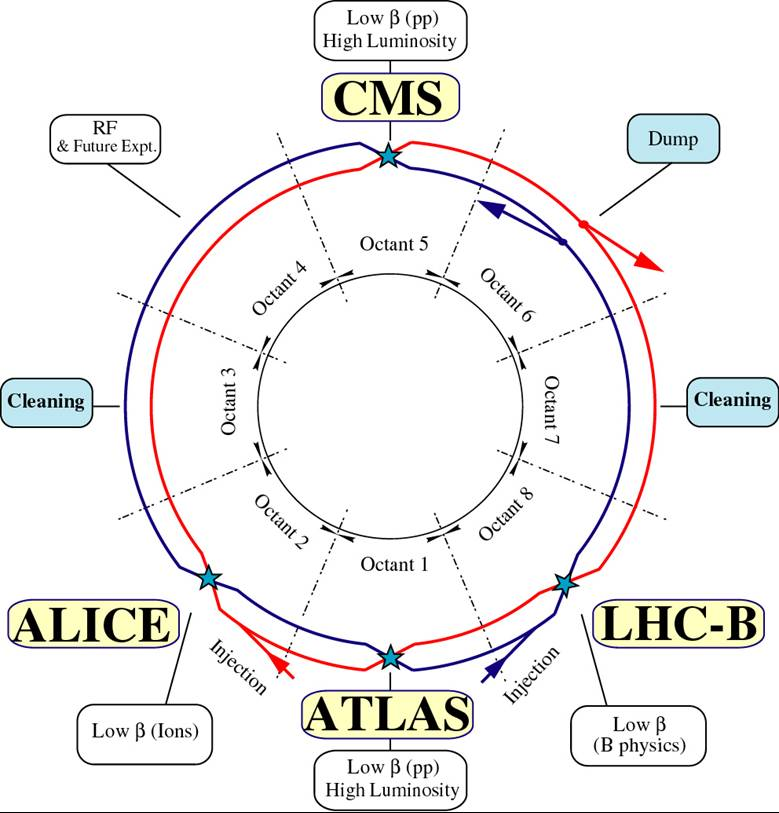
\includegraphics[width=0.95\textwidth]{figures/LHC/lhc-schematic.jpg}
	\caption{LHC geometry with arcs and straight sections.}
	\label{fig:LHCgeometry}
\end{figure}
\newline
{\bf ATLAS} (A Toroidal LHC Apparatus) and {\bf CMS} (Compact Muon Solenoid) are large general-purpose detectors having similar design and same physics goal. CMS detector will be described in detail in Section~\ref{sec:cms_experiment}. The main difference in the two is in their magnet systems. One additional choice that affects this is the momentum resoultion for muons. The momentum resolution for muons, $\Delta p_T/p_T$, are proportional to  $B^{-1}L^{-2}$, where B is magnetic field and L is distance of momentum measurement from the IP of detector. So, To imporve the momentum resoltuion there are two possible choices.

\begin{enumerate}
	\item Increase the magnetic field with compact design, or
	\item Work with low magnetic field with long lever arm, L
\end{enumerate}

There is also a third possiblity to increase the lever arm as well as magnetic field but it will increase the cost of detector by several factor. So, CMS chooses the first point, i.e., to increase the magnetic field with compact design\footnote{This is why there is word {\bf compact} in the name of CMS.} while ATLAS chooses the design with low magnetic field with logn lever arm.

% ATLAS has an eight toroidal magnets combined with a smaller inner solenoid while CMS has a powerful solenoid magnet only.

{\bf ALICE} (A Large Ion Collider Experiment) is a heavy-ion detector. It is specially designed for the study of strongly interacting matter at high densities in quark-gluon plasma phase.

{\bf LHCb} (Large Hadron Collider beauty) is made asymmetrically with respect to the IP of the detector. It is made specially to study the slight differences between the matter-antimatter through the study of b-quarks.

{\bf LHCf} (Large Hadron Collider forward) and {\bf TOTEM} (TOTal cross-section, Elastic scattering and diffraction dissociation Measurement at the LHC) are located near ATLAS and CMS respectively, for the study of forward physics.
% section experiments_at_the_lhc (end)

% %%%%%%%%%%%%%%%%%%%%%%%%%%%%%%%%%%%%%%%%%%%%%%%%%%%%%%%%%%%%%%%%%%
% \section{CMS Experiment} % (fold)
% \label{sec:cms_experiment}

% The CMS is a general-purpose detector at the LHC. It is built around a huge solenoid magnet. This takes the form of a cylindrical coil of superconducting cable that generates a field of 4 Tesla, about 100,000 times the magnetic field of the Earth. The field is confined by a steel ``yoke'' that forms the bulk of the detector's 12,500-tonne weight. The complete detector is 21 meters long, 15 meters wide and 15 meter high.

% \subsection{Detector Design} % (fold)
% \label{sub:detector_design}

% % subsection cms_detector_design (end)
% CMS\cite{paper:JINST:CMSCollaboration} detector is a general purpose deetector which consist of layers of material that exploit the different properties of particles to catch and measure the energy and momentum of each particles passing through it. So, CMS needs:
% \begin{itemize}
% 	\item a high quality central tracking system to give accurate momentum measurements with good efficienccy of offline tagging of b-jets and $\tau$'s.
% 	\item a high resolution ($\approx$ 1\% at 100 GeV) method to detect and measure electrons and photons (an electromagnetic calorimeter) and isolate them.
% 	\item a ``hermetic” hadron calorimeter, designed to entirely surround the collision and prevent particles from escaping along with fine lateral segmentation.
% 	\item a high performance system to detect and measure muons with good time and momentum resolution ($\approx$ 1\% at 100 GeV).
% \end{itemize}
% The CMS experiment has been built as a general purpose detector with excellent tracking and particle identification capabilities designed to fully explore the physics potential of the LHC. The CMS comprise the following sub-detectors:
% \begin{itemize}
% 	\item The inner tracking system is used for the identification and track measurement of charged particles.
% 	\item The electromagnetic calorimeter provides energy measurements. Electrons and photons deposit almost all of their energy in this sub-detector.
% 	\item Typically the interactions of hadronic jets imply that most of their energy is deposited after traversing more material than given by the electromagnetic calorimeter. The main energy component of these objects is measured with the hadronic calorimeter.
% 	\item The muon system identifies high energetic muons which can not be confined within the CMS experiment and measures their tracks and respective momenta.
% \end{itemize}



% %%%%%%%%%%%%%%%%%%%%%%%%%%%%%%%%%%%%%%%%%%%%%%%%%%%%%%%%%%%%%%%%%%
% %%%%%%%%%%%%%%%%%%%%%%%%%%%%%%%%%%%%%%%%%%%%%%%%%%%%%%%%%%%%%%%%%%
% \subsection{CMS sub-systems} % (fold)
% \label{sub:cms_sub_systems}

% % subsection cms_sub_systems (end)

% %%%%%%%%%%%%%%%%%%%%%%%%%%%%%%%%%%%%%%%%%%%%%%%%%%%%%%%%%%%%%%%%%%
% %%%%%%%%%%%%%%%%%%%%%%%%%%%%%%%%%%%%%%%%%%%%%%%%%%%%%%%%%%%%%%%%%%
% \subsubsection{Tracker} % (fold)
% \label{ssub:tracker}
% % subsection tracker (end)

% %%%%%%%%%%%%%%%%%%%%%%%%%%%%%%%%%%%%%%%%%%%%%%%%%%%%%%%%%%%%%%%%%%
% %%%%%%%%%%%%%%%%%%%%%%%%%%%%%%%%%%%%%%%%%%%%%%%%%%%%%%%%%%%%%%%%%%
% \subsubsection{The Electromagnetic Calorimeter} % (fold)
% \label{sub:the_electromagnetic_calorimeter}
% % subsection the_electromagnetic_calorimeter (end)

% %%%%%%%%%%%%%%%%%%%%%%%%%%%%%%%%%%%%%%%%%%%%%%%%%%%%%%%%%%%%%%%%%%
% %%%%%%%%%%%%%%%%%%%%%%%%%%%%%%%%%%%%%%%%%%%%%%%%%%%%%%%%%%%%%%%%%%
% \subsubsection{The Hadronic Calorimeter} % (fold)
% \label{sub:the_hadronic_calorimeter}
% % subsection the_hadronic_calorimeter (end)

% %%%%%%%%%%%%%%%%%%%%%%%%%%%%%%%%%%%%%%%%%%%%%%%%%%%%%%%%%%%%%%%%%%
% %%%%%%%%%%%%%%%%%%%%%%%%%%%%%%%%%%%%%%%%%%%%%%%%%%%%%%%%%%%%%%%%%%
% \subsubsection{The Muon System} % (fold)
% \label{sub:the_muon_system}

% % subsection the_muon_system (end)

% % section cms_experiment (end)

% %%%%%%%%%%%%%%%%%%%%%%%%%%%%%%%%%%%%%%%%%%%%%%%%%%%%%%%%%%%%%%%%%%
% \section{CMS Trigger and Data Acquisition system} % (fold)
% \label{sec:cms_trigger_and_data_acquisition_system}

% % section cms_trigger_and_data_acquisition_system (end)

% %%%%%%%%%%%%%%%%%%%%%%%%%%%%%%%%%%%%%%%%%%%%%%%%%%%%%%%%%%%%%%%%%%
% \section{CMS Offline Computing} % (fold)
% \label{sec:cms_offline_computing}

% section cms_offline_computing (end)




% \begin{figure}[!htbp]
% 	\centering
% 	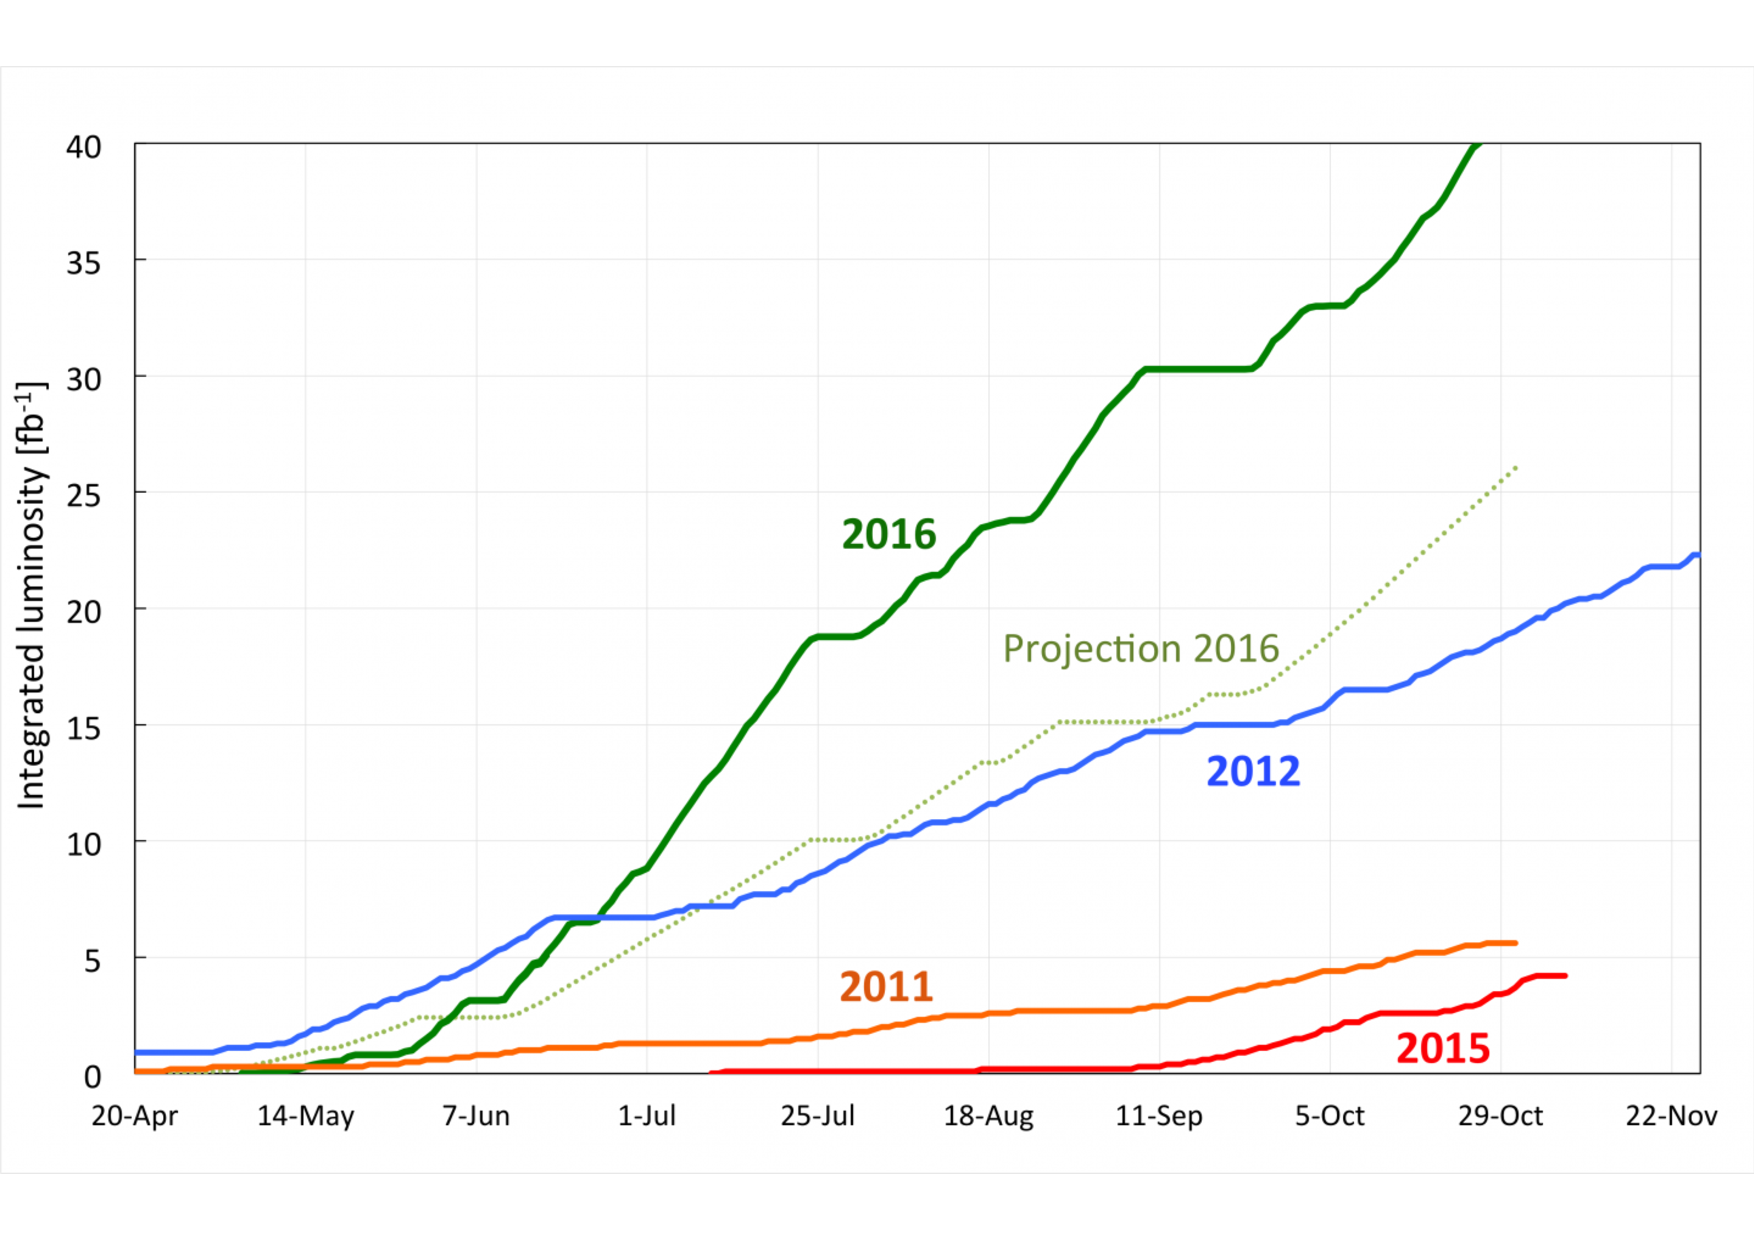
\includegraphics[width=0.95\textwidth]{figures/lumi-proj-2016-final-v2}
% 	\caption{The integrated luminosity of the LHC with proton-proton collisions in 2016 compared to previous years. Luminosity is a measure of a collider’s efficiency and is proportional to the number of collisions. The integrated luminosity achieved by the LHC in 2016 far surpassed expectations and is double that achieved at a lower energy in 2012. (Image : CERN)\todo[inline]{Update the caption.}}
% 	\label{fig:lumi-proj-2016-final-v2}
% \end{figure}



% \section{Other Information to be organized}



% The interaction in HEP experiments are characterized mainly by the center of mass energy along with type and number of particles.


% Because of limited geometrical space in LHC ring the beam pipe was designed as a ``twin-aperture" magnets, where superconducing ring is housed in a common return yoke and cryostat.

% chapter the_lhc_and_cms_machine (end)